% ******** Приклад оформлення документа за ДСТУ 3008-95 ********
% ******************** автор: Тавров Д. Ю. *********************

% зазначаємо стильовий файл, який будемо використовувати
\documentclass{udstu}

% починаємо верстку документа
\begin{document}

% створимо титульний аркуш
% за допомогою спеціальної команди
% \maketitlepage{params},
% де params --- це розділені комами пари "параметр={значення}"
\maketitlepage{
% StudentName --- прізвище, ініціали студента
	StudentName={Скорденко Д. О.},
% StudentMale --- стать студента (true, якщо чоловік, false --- якщо жінка)
	StudentMale=true,
% StudentGroup --- група студента
	StudentGroup={КМ-01},
% Title --- назва
	Title={Звіт\\із лабораторної роботи №5\\із дисципліни \invcommas{Розподілені і хмарні обчислення}},
% SupervisorDegree --- науковий ступінь, учене звання керівника роботи
% якщо наукового ступеня немає, можна відповідний рядочок пропустити
	SupervisorDegree={доцент кафедри ПМА},
% SupervisorName --- прізвище, ініціали керівника роботи
	SupervisorName={Ліскін В. О.}
}

% створюємо зміст
\tableofcontents

% створюємо вступ
\intro

\paragraph{\textbf{Мета:}} розпаралелити метод обчислення константи \pi.


% створюємо перший розділ роботи
\chapter{Основна частина}
\label{chap:1}

\paragraph{\textbf{Опис програми:}}

Для реалізації паралелізму буде використовуватись 'Rayon'.

\chapter{Опис програми [Тестовий приклад]}
\label{chap:3}

\begin{figure}[!htp]
	\centering
	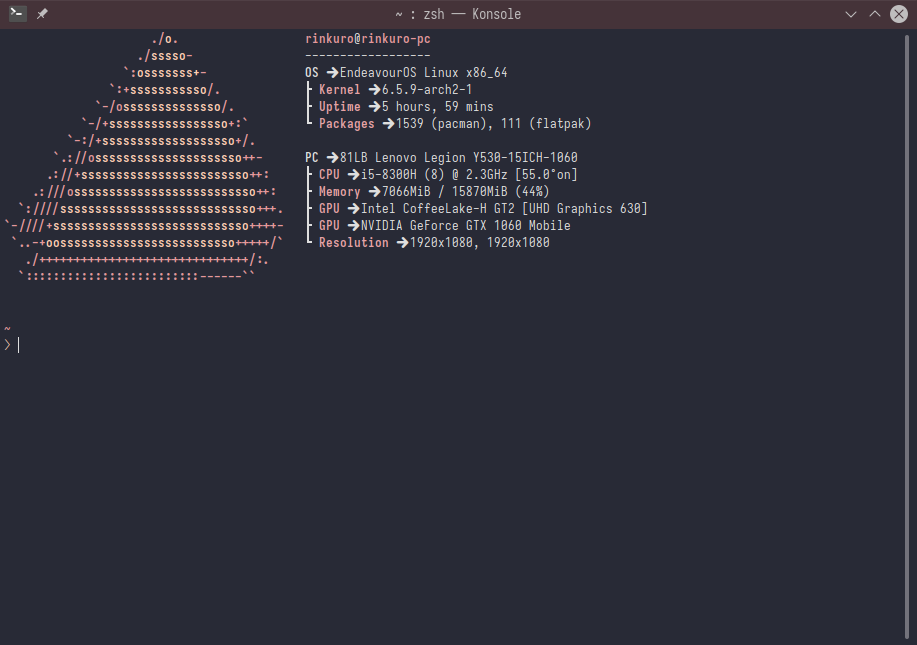
\includegraphics[scale=0.5]{PNG/system-specs.png}
	\caption{Характеристики системи}
	\label{fig:figure1}
\end{figure}

\begin{figure}[!htp]
	\centering
	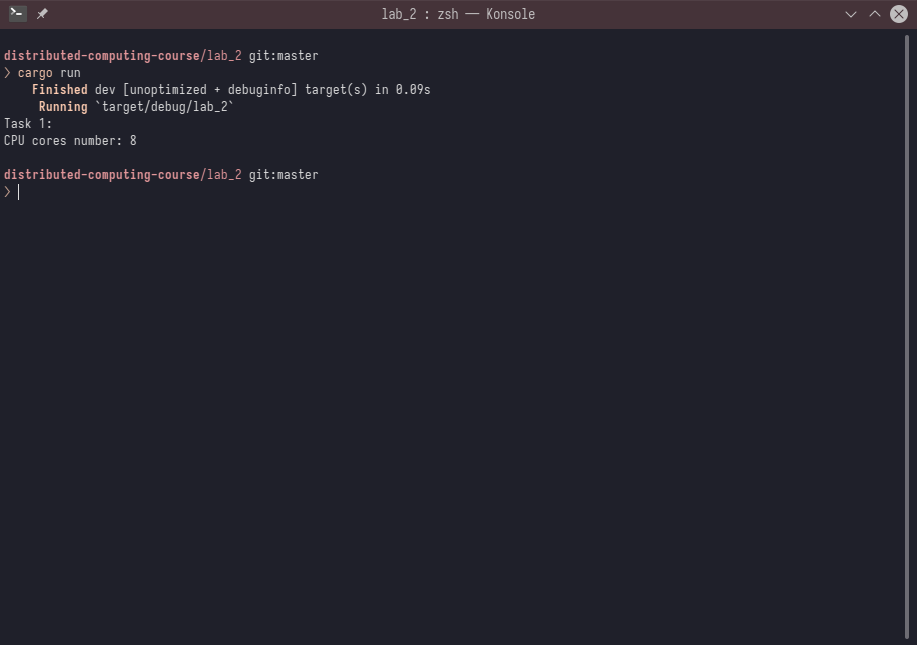
\includegraphics[scale=0.5]{PNG/thread-num-test.png}
	\caption{К-сть ядер процесора}
	\label{fig:figure1}
\end{figure}

\begin{center}
\captionof{table}{Порівняння швидкодії}
\resizebox{\textwidth}{!}{
\begin{tabular}{ | c | c | c | }
	\hline
	Метод & Результат \\
	\hline
	Редукція & 3.1415928535894384 \\
	Монте-Карло & 3.1415868 \\
	\hline
\end{tabular}
}
\end{center}

% створюємо Висновки
\conclusions

Було розпаралелено два методи обчислення числа \pi.

Метод Монте-Карло виявився менш точним ніж метод редукції.

\append{Код лістінги}

\paragraph{\textsc{*Примітка:}}
У код лістингах при копіюванні втрачається форматування (не копіюються пробіли).
Файли прикріплено до цього pdf (вкладка "прикріплені файли").

\captionof{listing}{constcalc.rs}
\embedfile[filespec=constcalc.rs]{../src/constcalc.rs}
\inputminted{rust}{../src/constcalc.rs}

\captionof{listing}{lib.rs}
\embedfile[filespec=lib.rs]{../src/lib.rs}
\inputminted{rust}{../src/lib.rs}

\captionof{listing}{main.rs}
\embedfile[filespec=main.rs]{../src/main.rs}
\inputminted{rust}{../src/main.rs}

\end{document}
